\documentclass[a4paper, 12pt]{article}
\usepackage{pgfplots, mathtools}

%% Listings With Code-Styling and Grey Background
\usepackage{float, listings} 
\lstset{						% Global Listing settings
	language=Verilog,
	numbers=left,
	numberstyle=\tiny\color{gray},
%	firstnumber=1,
	numberfirstline=true,
	stepnumber=1,
	tabsize=2,
	breaklines=true,
}
\usepackage{xcolor, mdframed, graphicx}
\definecolor{code-gray}{gray}{0.93}

%% Make specific pages landscale for larger figures
\usepackage{pdflscape}

%% Custom FSM's
\usepackage{tikz}
\usetikzlibrary{automata, positioning, arrows}
\tikzset{very thick, ->, >=stealth', node distance=6cm, every state/.style={thick, fill=gray!10}, initial text=$ $}

%% Automatic Word Formatting
\usepackage{xspace}
\newcommand*{\Vivado}{\textit{Vivado}\xspace} % Italicize Vivado
\newcommand*{\SV}{\textbf{SystemVerilog}\xspace} % Bold SystemVerilog

%% Clickable links in the output PDF
\usepackage{hyperref}
\hypersetup{colorlinks=true, linktoc=all, linkcolor=black}

%% Figure Numbering Within Sections
\let\counterwithout\relax
\let\counterwithin\relax
\usepackage{chngcntr}
\counterwithin{figure}{section}

%% Macros for logic timing diagrams
\newcounter{wavenum}
\setlength{\unitlength}{1cm}
% advance clock one cycle, not to be called directly
\newcommand*{\clki}{
  \draw (t_cur) -- ++(0,.3) -- ++(.5,0) -- ++(0,-.6) -- ++(.5,0) -- ++(0,.3)
    node[time] (t_cur) {};
}
\newcommand*{\bitvector}[3]{
  \draw[fill=#3] (t_cur) -- ++( .1, .3) -- ++(#2-.2,0) -- ++(.1, -.3)
                         -- ++(-.1,-.3) -- ++(.2-#2,0) -- cycle;
  \path (t_cur) -- node[anchor=mid] {#1} ++(#2,0) node[time] (t_cur) {};
}
% \known{val}{length}
\newcommand*{\known}[2]{
    \bitvector{#1}{#2}{white}
}
% \unknown{length}
\newcommand*{\unknown}[2][XXX]{
    \bitvector{#1}{#2}{black!20}
}
% \bit{1 or 0}{length}
\newcommand*{\bit}[2]{
  \draw (t_cur) -- ++(0,.6*#1-.3) -- ++(#2,0) -- ++(0,.3-.6*#1)
    node[time] (t_cur) {};
}
% \unknownbit{length}
\newcommand*{\unknownbit}[1]{
  \draw[ultra thick,black!50] (t_cur) -- ++(#1,0) node[time] (t_cur) {};
}
% \nextwave{name}
\newcommand{\nextwave}[1]{
  \path (0,\value{wavenum}) node[left] {#1} node[time] (t_cur) {};
  \addtocounter{wavenum}{-1}
}
% \clk{name}{period}
\newcommand{\clk}[2]{
    \nextwave{#1}
    \FPeval{\res}{(\wavewidth+1)/#2}
    \FPeval{\reshalf}{#2/2}
    \foreach \t in {1,2,...,\res}{
        \bit{\reshalf}{1}
        \bit{\reshalf}{0}
    }
}

% \begin{wave}[clkname]{num_waves}{clock_cycles}
\newenvironment{wave}[3][clk]{
  \begin{tikzpicture}[draw=black, yscale=.7,xscale=1]
    \tikzstyle{time}=[coordinate]
    \setlength{\unitlength}{1cm}
    \def\wavewidth{#3}
    \setcounter{wavenum}{0}
    \nextwave{#1}
    \foreach \t in {0,1,...,\wavewidth}{
      \draw[dotted] (t_cur) +(0,.5) node[above] {t=\t} -- ++(0,.4-#2);
      \clki
    }
}{\end{tikzpicture}}

%$ Specific Line Breaks
% See https://tex.stackexchange.com/questions/26174/ for details
\usepackage[british]{babel} 

%% Page Margins
\usepackage[margin=1.00in]{geometry}

%% Beginning of Document
\begin{document}
\counterwithin{lstlisting}{section} % Listings are numbered within sections
% Title
\title{ECE 440 - Project \#10}
\author{Collin Heist}
\date{\today}
\maketitle

% Table of Content and Listings
\pagenumbering{roman}
\tableofcontents
\renewcommand{\listfigurename}{Figures}
\listoffigures
\lstlistoflistings
\newpage
\pagenumbering{arabic}

\section{Design}
I based my factorial (without addition) module on the algorithm we designed on the exam / was shown in class.
I started with a three-state FSM, having a reset, compute, and done state. However, I found that by using a Mealy FSM and only asserting the \textbf{done} signal as a single-clock pulse (not staying high until a new \textbf{start} or \textbf{reset}) I was able to remove the done state altogether. The FSM for this module is shown below, in \textbf{Figure~\ref{fig:fsm-factorial}}.

\begin{figure}[H]
\centering
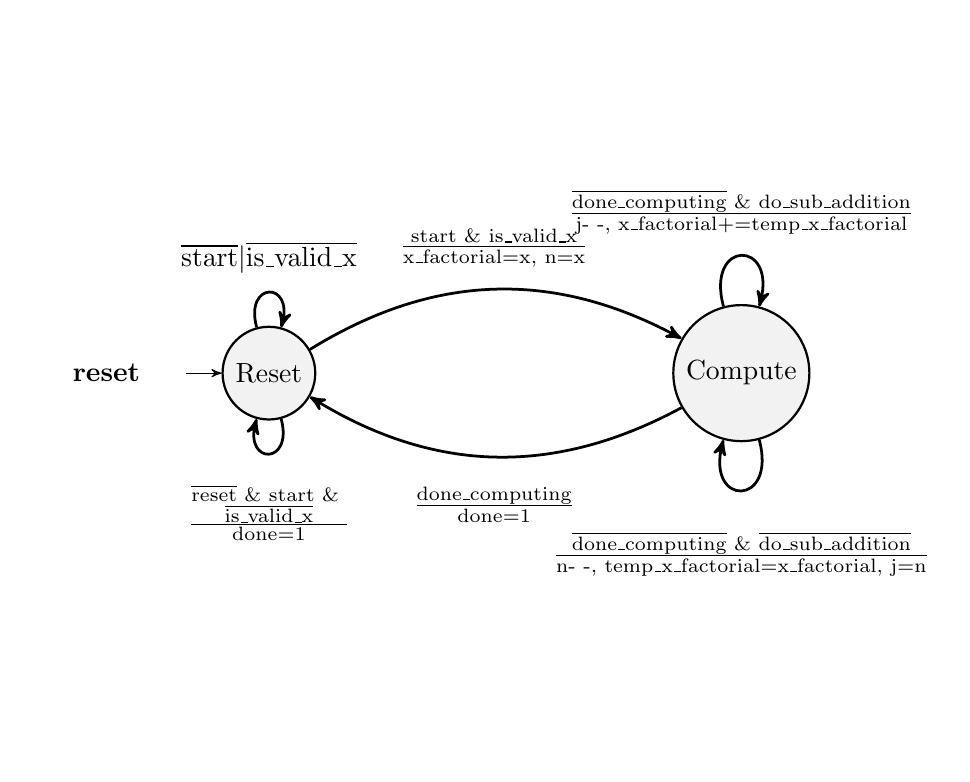
\begin{tikzpicture}[initial text=\textbf{reset}, every node/.style={circle, minimum size=2cm, align=center}]
	\node[initial, state] (Reset) {Reset};
	\node[state, right of=Reset] (Compute) {Compute};
	\draw[->, line width=0.35mm]
		(Reset) edge[loop above, looseness=5] node[yshift=-0.85cm]{$\overline{\text{start}} \vert \overline{\text{is\_valid\_x}}$} (Reset)
		(Reset) edge [loop below, looseness=5] node[yshift=0.5cm]{$\frac{\substack{\overline{\text{reset}}\text{ \& start \& }\\ \overline{\text{is\_valid\_x}}}}{\text{done=1}}$} (Reset)
		(Reset) edge[bend left, above] node[yshift=-0.85cm]{$\frac{\text{start \& is\_valid\_x}}{\text{x\_factorial=x, n=x}}$} (Compute)
		(Compute) edge[loop above, looseness=5] node[yshift=-1.80cm]{$\frac{\overline{\text{done\_computing}}\text{ \& do\_sub\_addition}}{\text{j- -, x\_factorial+=temp\_x\_factorial}}$} (Compute)
		(Compute) edge[loop below, looseness=5] node[yshift=1.75cm]{$\frac{\overline{\text{done\_computing}}\text{ \& }\overline{\text{do\_sub\_addition}}}{\text{n- -, temp\_x\_factorial=x\_factorial, j=n}}$} (Compute)
		(Compute) edge[bend left, below] node[yshift=0.60cm]{$\frac{\text{done\_computing}}{\text{done=1}}$} (Reset);
\end{tikzpicture}
\caption{Factorial Finite State Machine}
\label{fig:fsm-factorial}
\end{figure}

Fairly straightforward (as is the algorithm its based on) the FSM only leaves the \textbf{compute} state when the module is done computing the result, at which point done is asserted. The two loops on the \textbf{compute} state are the two looping operations of the algorithm -- either the inner or outer ones. The control signals for this FSM are \textbf{done\_computing}, \textbf{do\_sub\_addition}, and \textbf{is\_valid\_x}.

These are fairly self-explanatory, but \textbf{is\_valid\_x} just prevents the module from attempting to compute a number with no definable factorial (through this algorithm, i.e. $x\leq 0$), or wasting clock cycles on $x=1$. If a \textbf{start} is initiated but an invalid $x$ is entered, then the \textbf{x\_factorial} result is automatically assigned to 1 - saving any \textit{computation}. The \textbf{do\_sub\_addition} control signal is used to control the 2nd of the \textit{nested} loops in the computation state. For all values of $j <1$, no more iterations of the loop are required. In a similar vein, \textbf{done\_computing} is detected when the number of remaining loops ($n$) is equal to 1 -- meaning all operations are done and \textbf{done} can be asserted.

\section{Tribulations}
\label{sec:tribulations}
With the removal of the SDK portion of this project, I did not struggle with anything in the remaining project. When the SDK part \textit{was} a requirement, I struggled quite a bit with making the clock and reset signals external as a part of the bitstream generation, but otherwise had no hiccups.

\begin{landscape}
\section{Simulations}
I tested various values of $x$ while designing the module, but for simulations I created a testbench (shown in \textbf{Listing~\ref{lst:factorial-testbench}}) to just test $x=4, 9, $ and $12$. The results are shown below:

\begin{figure}[H]
\centering
\includegraphics[width=0.80\paperheight, keepaspectratio=true]{Sources/post-synth-time-4.jpg}
\caption{Full waveform for the post-synthesis timing simulation, showing $4!=24$.}
\label{fig:behav-codon-reader}
\includegraphics[width=0.80\paperheight, keepaspectratio=true]{Sources/post-synth-time-9.jpg}
\caption{Full waveform for the post-synthesis timing simulation, showing $9!=362,880$.}
\label{fig:behav-codon-reader}
\includegraphics[width=0.80\paperheight, keepaspectratio=true]{Sources/post-synth-time-12.jpg}
\caption{Full waveform for the post-synthesis timing simulation, showing $12!=479,001,600$.}
\label{fig:behav-codon-reader}
\end{figure}

Although the larger factorials (specifically $x=12$) take fairly long to compute, the end result of \textbf{x\_factorial} is correct in all the tested cases (as can be seen on the left bar of the final two images).
\end{landscape}

\section{Source Code}
\begin{mdframed}[backgroundcolor=code-gray, roundcorner=10pt, innerleftmargin=25, innertopmargin=5, innerbottommargin=5]	
\lstinputlisting[caption=Factorial Module, label={lst:factorial}]{Sources/factorial.sv}
\end{mdframed}

\begin{mdframed}[backgroundcolor=code-gray, roundcorner=10pt, innerleftmargin=25, innertopmargin=5, innerbottommargin=5]	
\lstinputlisting[caption=Factorial Testbench, label={lst:factorial-testbench}]{Sources/factorial_tb.sv}
\end{mdframed}

\end{document}